\documentclass[12pt, a4paper]{article}
%IMPORTS
\usepackage{polski}
\usepackage[utf8]{inputenc}
\usepackage[a4paper, total={15cm, 24cm}]{geometry}
\usepackage[T1]{fontenc}

\usepackage{graphicx}
\usepackage[inkscapeformat=pdf]{svg}

\usepackage{url}
\usepackage{hyperref}
\hypersetup{
    colorlinks=true,
    linkcolor=blue,
    filecolor=magenta,      
    urlcolor=cyan,
    pdftitle={Overleaf Example},
}

\usepackage{amsmath}
\usepackage{bytefield}
\usepackage{siunitx}
\usepackage{minted}
\usepackage{circuitikz}
\usetikzlibrary{decorations.shapes}

\usepackage{biblatex}
\addbibresource{references.bib}

\graphicspath{{img/}}

\title{
	Generator sygnału \qty{1}{\kHz}\\
	\large Raport Techniczny
}

\author{Szymon Januszek, \texttt{szymon\_j@tutanota.com}}

\date{Kwiecień 2023}

\begin{document}
\normalfont
\fontfamily{lmtt}
\maketitle
\hrule

\begin{abstract}
	Dokumen zawiera opis budowy i działania generatora przebiegu \qty{1}{\kHz}.
\end{abstract}

\begin{center}
	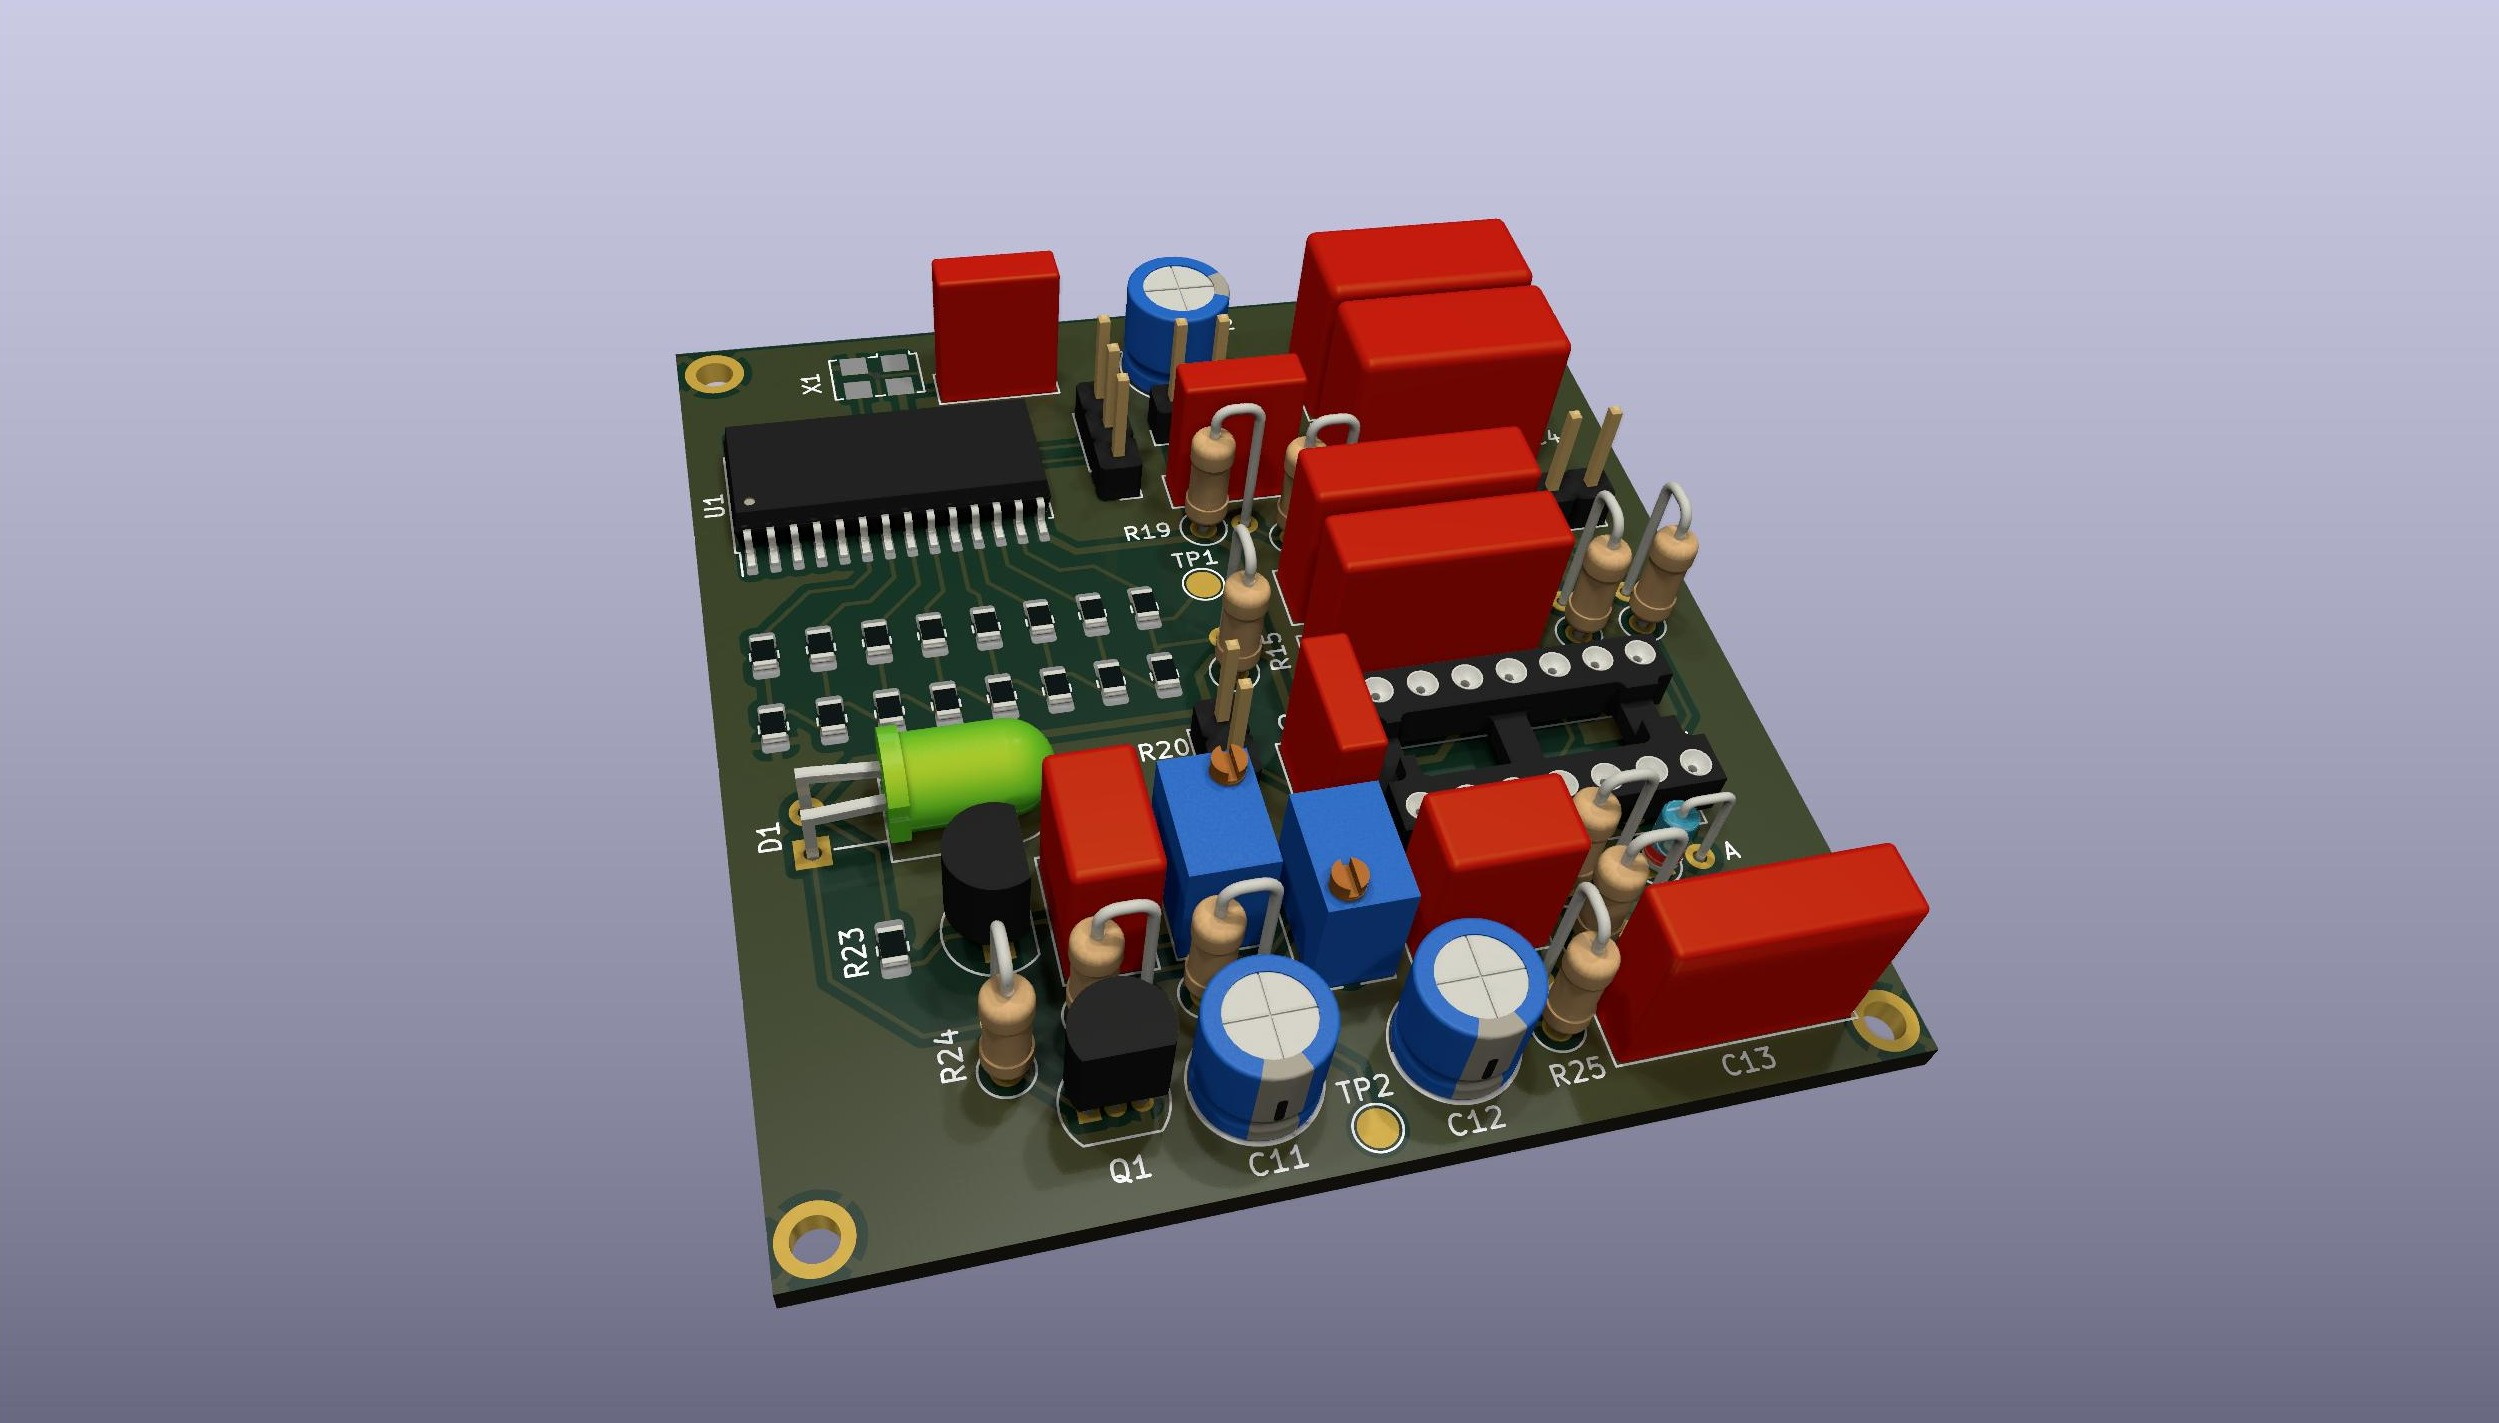
\includegraphics[width=0.9\textwidth]{img/board_render_1.jpg}
\end{center}

%TODO: fancy graphics

\newpage

\tableofcontents

\newpage

\section{Bezpośrednia synteza cyfrowa}

Aby wygenerować maksymalnie stabilny i dokładny względem częstotliwości sygnał, 
zdecydowałem się na wykorzystanie techniki \verb|Bezpośredniej Syntezy Cyfrowej|, 
gdzie mikroprocesor wraz z układem Przetwornika Cyfrowo-Analogowego (DAC) generuje sygnał zbliżony do sygnału oczekiwanego. 
Umożliwia to zastosowanie wysokiej jakości generatora kwarcowego, o precyzji rzędu 50ppm\footnote{Części na milion}, 
w całym zakresie temperatur. Oznacza to, iż częstotliwość uzyskanego sygnału nie będzie odbiegać o więcej niż $\pm$\qty{50}{\mHz} od wartości oczekiwanej. 

\subsection{Mikrokontroler}
Jako główny mikrokontroler wybrany został układ \textbf{AVR32DA28}\cite{avr-datasheet} należący do rodziny 8-bitowych układów AVR.
W porównaniu ze starszymi generacjami, producent dopuszcza pracę układu przy częstotliwościach przekraczających \qty{8}{\MHz} z napięciem \qty{3}{\volt}.
Jednocześnie dokonana została unifikacja modelu pamięci, co okaże być się przydatne przy pisaniu oprogramowania(\ref{sec:impl}).

\subsection{Przetwornik Cyfrowo-Analogowy}
Do implementacji przetwornika zrealizowany został układ drabinki R-2R (Rys.\ref{fig:r-2r-ladder}),
umożliwiając łatwą zmianę wartości liczbowej, przedstawionej jako liczba binarna na pinach mikrokontrolera, 
na ułamek napięcia zasilania.

\begin{figure}[h]
	\centering

	\begin{circuitikz}[scale=0.9]
		\def\n{2}
	
		\node (ground) at (-2, 0) {};
		\node (Vcc) at (0, 3) {};
	
		\foreach \contact in {0,...,\n}
		{
			% Define contacts for each bits
			\node (up contact \contact)    at ($({2*\contact}, 2)$) {};
			\node (down contact \contact)  at ($({2*\contact}, 0)$) {};
	
			% Draw R resistors and manage the a_{n-0} case
			\ifnum \contact>0
	
				\node (up contact -\contact)   at ($({2+4*\n-2*\contact}, 2)$) {};
				\node (down contact -\contact) at ($({2+4*\n-2*\contact}, 0)$) {};
	
				\draw (down contact \contact) to [R=R, *-*] ($(down contact \contact)-(2, 0)$);
				\draw (up contact -\contact) node[anchor=south] {$a_{n-\contact}$};
				\draw (down contact -\contact)   to [R=2R, *-o]  (up contact -\contact);
			\fi
			\ifnum \contact>1
				\draw ($(down contact -\contact)+(2, 0)$) to [R=R, *-*] (down contact -\contact);
			\fi
	
			% Draw 2R resistors
			\draw (down contact \contact)    to [R=2R, *-o]  (up contact \contact)
											 node[anchor=south] {$a_{\contact}$};
		}
		
		% Draw ground and Vout
		\draw (down contact 0)  to [R=2R, *-*] (ground) node[ground] {}
			  (down contact -1) to [short, *-o] ($(down contact -1)+(1,0)$)
								node[anchor=west]  {$V_{wyj}$};
	
		% Draw ldots
		\draw[fill=black,decorate,decoration={shape backgrounds,shape=circle,shape size=1mm}]
						($0.67*(down contact \n)+0.33*(down contact -\n)$) -- ($0.33*(down contact \n)+0.67*(down contact -\n)$);
		\draw[fill=black,decorate,decoration={shape backgrounds,shape=circle,shape size=1mm}]
						($0.67*(up contact \n)+0.33*(up contact -\n)$) -- ($0.33*(up contact \n)+0.67*(up contact -\n)$);
	\end{circuitikz}
	
	\caption{Schemat drabiny R-2R \cite{r-2r-image-wiki}}
	\label{fig:r-2r-ladder}
	
\end{figure}

Napięcie na węźle wyjściowym przetwornika można opisać w następujący sposób:

\[
	V_{wyj}=V_{ref} \times \frac{a_0 \times 2^0 + a_1 \times 2^1 + a_2 \times 2^2 + ... + a_{N - 1} \times 2^{N- 1}}{2^N}
\]

Jak widać, przy $N=8$, przetwornik ten pozwala na uzyskanie 256 różnych wartości. Dla $V_{ref}=\qty{3}{\volt}$,
oznacza to, iż różnica pomiędzy dwoma dowolnymi stopniami wynosi ok. \qty{11,72}{\mV}.

Co ciekawe, okazuje się, iż impedancja wyjściowa takiego układu jest stała dla każdego poziomu
\footnote{
	Wynika to z Twierdzenie Thévenina, zakładającego zerową impedancję źródła oraz mikrokontrolera. 
	W rzeczywistości ich wartości są znacznie mniejsze od wartości R.
}.

Aby zachować użyteczność najniższych bitów, precyzja wykorzystanych rezystorów musi być lepsza niż
$\frac{1}{2^N} \times 100\unit{\percent} \approx \qty{0,3}{\%}$. Na szczęście,
w sprzedaży dostępne są rezystory przeznaczone do montażu powierzchniowego o precyzji \qty{0,1}{\%}.

\subsection{Analiza zniekształceń przetwornika}

Sygnał generowany w ten sposób nie opowiada jednak perfekcyjnej sinusoidzie (Rys. \ref{fig:sine-stepped}).
Obecne jest tzw. zniekształcenie kwantyzacji, wynikające z faktu, iż sygnał złożony jest 
z serii dyskretnych wartości. Jednak jeśli dokładnie przyjrzymy się różnicy pomiędzy naszym sygnałem
a idealnej sinusoidzie, to okaże się, że następna składowa generowanego sygnału ma częstotliwość $f_1 = f_0 \times N_{smpl}$.

Co więcej, stosunek mocy całego sygnału do mocy wyższych składowych dla konwertera z N-bitami wynosi
\begin{equation}
	SQR = 1.76 + 6.02 \times N (dB)
\end{equation}

Przy $N=8$ oraz $N_{smpl}=1024$ oznacza to iż całkowita moc zniekształceń względem sygnału fundamentalnego wynosi \qty{-50}{\dB}, 
oraz jest rozłożona w paśmie megahercowym.

\begin{figure}[h]
	\centering
	\includegraphics[width=0.6\textwidth]{sine_steps.png}
	%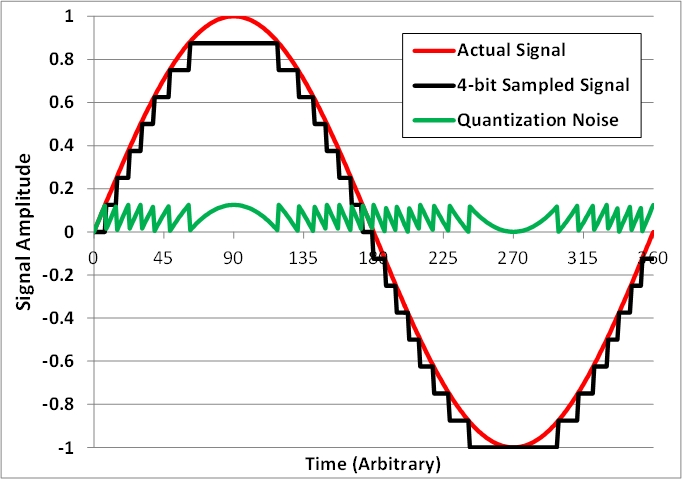
\includegraphics[width=0.55\textwidth]{img/qunatization_error_fig.jpg}
	\caption{Przebieg sinusoidy generowanej przy pomocy przetwornika R-2R.}
	\label{fig:sine-stepped}
\end{figure}

\section{Kształtowanie}
Mimo wszystko należy usunąć składowe wyższej częstotliwości. Funkcje tą realizuje kondensator \verb|C2| (Rys. \ref{fig:filter}).

Dodatkowo, rzeczywiste wzmacniacze operacyjne nie są wstanie generować sygnałów bardzo bliskich $<\qty{300}{\mV}$ szyn zasilania.
Tłumienia tego dokonują \verb|C1, R1, R2|, zachowując wartość środkową na poziomie \qty{1,5}{\V}

\begin{figure}[h]
	\centering
	\includesvg{img/filter.svg}
	\caption{Schemat filtru}
	\label{fig:filter}
\end{figure}

\section{Kontrola Amplitudy}

Ostatnią zmienną którą należy rozpatrzyć jest amplituda sygnału wyjściowego. Na tym etapie poziom sygnału jest wyższy od oczekiwanej wartości
\qty{0,5}{\V}. Potrzebna jest więc metoda dokładnego tłumienia, nie wprowadzająca dodatkowych zniekształceń i zakłócenia.

Rozwiązanie oparte o nawet precyzyjny potencjometr pozostaje jednak wrażliwe na zmianę absolutnej wartości napięcia zasilania,
czy też dryft elementów związany ze zmianą temperatury.

Tak więc, niezbędny jest układ aktywnie korygujący amplitudę sygnału.
Cyfrowa implementacja takiego rozwiązania nie wchodzi w gre, 
ponieważ przetwornik DAC nie posiada wystarczającej głębokości bitowej. 
Stąd też, proponuję rozwiązanie w pełni analogowe.

Przy użyciu wzmacniaczy operacyjnych możemy uzyskać pętle sprzężenia zwrotnego, 
korygującą amplitude sygnału względem stałego napięcia odniesienia.
Do realizacji tego rozwiązania potrzebujemy następujących elementów.

\subsection{Pomiar amplitudy}
Konieczny jest pomiar amplitudy sygnału wyjściowego. \
To tego celu służy tzw. Detektor szczytowy (Rys. \ref{fig:peak-detector-schematic}). 

\begin{figure}[h]
	\centering
	%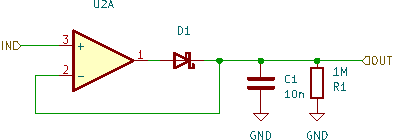
\includegraphics{img/peak_detector.pdf}
	\includesvg{img/peak_detector.svg}
	\caption{Przykładowy schemat połówkowego detektora szczytowego}
	\label{fig:peak-detector-schematic}
\end{figure}

\subsection{Element sprzęgający}
Wymagany jest układ umożliwiający tłumienie sygnału zmiennego względem sygnału sterującego:

\begin{equation}
	V_{wyj} \propto \frac{V_{wej}}{V_{ster}}
	\label{eq:coupling_1}
\end{equation}

Fizyczna implementacja takiego układu okazuje się być niebanalna.
Możliwy jest układ realizujący operacje mnożenia wartości sygnałów. 
Jego realizacja jednak jest wysoce złożona i wymaga relatywnie dużo części.

Alternatywna metoda wykorzystuje element zmieniający swój opór elektryczny względem jakiegoś innego czynnika.
Przykładem historycznej realizacji takiego układu jest zastosowanie niewielkiej łapmy żarowej,
której opór włókna jest wprost proporcjonalny do jego temperatury.

Istnieje jednak znacznie prostsze i wydajniejsze rozwiązanie.

Popularnym elementem o zmiennym oporze jest fotorezystor. W przeciwieństwie do 
np. tranzystorów jFET, przy stałym natężeniu światła, zachowuje się on jak faktyczny rezystor,
tzn. prąd przepływający jest wprost proporcjonalny do przyłożonego napięcia
$I \propto V$, tym samym jego zastosowanie nie wprowadzi zniekształceń mogących wynikać
z nie liniowości elementów półprzewodnikowych.

Tak więc, jeśli zamknie się fotorezystor w obudowie światłoszczelnej wraz z diodą LED,
uzyskamy układ o zmiennym oporze elektrycznym, kontrolowany przez prąd diody\footnote{Zakładam $\phi \propto I$}.

\begin{equation}
	R \propto \frac{1}{I_{Led}}
\end{equation}

Umożliwia to łatwą implementacje układu sprzężenia (Eq. \ref{eq:coupling_1}). 

Co prawda powyższy model ignoruje fakt,
iż tak na prawdę opór fotorezystora zależny jest wykładniczo od natężenia padającego światła
$R = \left(\frac{1}{\phi}\right)^A$. Nie stanowi jednak to dużego problemu ponieważ układ ten znajduje się w 
pętli sprzężenia zwrotnego.

\begin{equation}
	R \propto \frac{1}{(I_{Led})^A}
\end{equation}

\subsection{Źródło odniesienia}
W tym momencie potrzebne jest jedynie stabilne oraz dostrajalne źródło napięcia odniesienia.
Do tego celu z zupełności wystarczy układ LM4041 wraz z precyzyjnym potencjometrem.

\subsection{Dostrajanie}
Szczególnie trudnym okazało się zapewnienie stabilnej pracy układu. 
Wartości elementów w pętli kompensacji zostały w większości dobrane empirycznie.
Konieczne było zastosowanie dużej pojemności kondensatorów elektrolitycznych, 
ze względu na duży czas propagacji sygnału przez resztę układu.

\section{Oprogramowanie}
\label{sec:impl}
Czas przejść do opisu kodu źródłowego.
W pliku \verb|sine_tab.cpp| znajduje się definicja tabeli funkcji sinus. Składa się ona z $N_{smpl}=1024$ próbek, a wartość \verb|i|-tej próbki 
zdefiniowana jest w następujący sposób:

\begin{equation}
	f(i) = 2^N + \left\lfloor (2^N - 1) \times \sin \left(\frac{2 \pi \times i}{N_{smpl}}\right)\right\rceil
\end{equation}
\begin{equation}
	f(i) = 128 + \left\lfloor 127 \times \sin \left(\frac{2 \pi \times i}{1024}\right)\right\rceil
\end{equation}

Każda próbka jest 8-bitową liczbą całkowitą z zakresu $\in \{1 \dots 255\}$, jednocześnie tabela przedstawia cały jeden okres funkcji sinus,
poza wartością $\sin (2 \pi)$. Następną próbkę stanowi wartość $\sin (0)$. Dzięki temu reprodukowany sygnał nie zawiera błędów co okres.

Zadaniem oprogramowania mikrokontrolera pozostaje wczytanie kolejnych wartości z pamięci,
a następnie ustawienie pinów na odpowiedni stan. Wykorzystując 8-bitową naturę architektury AVR
możliwe jest ustawienie stanu całego rejestru (tj. grupy 8 pinów) poprzez pojedynczy zapis do 
obszaru peryferialnego pamięci (Linia \ref{code:set_pin_reg})

W tym miejscu napotykamy jednak pewien problem, synteza powyższego sygnału wymaga produkcji ponad miliona próbek na sekundę,
tym czasem zastosowany mikroprocesor jest przystosowany do pracy przy częstotliwości nie przekraczających \qty{24}{\MHz}.
Przy zastosowanym generatorze kwarcowym o częstotliwości pracy \qty{12,288}{\MHz} oznacza to, że mamy dokładnie \textbf{12} cykli maszynowych
na wygenerowanie następnej próbki, co więcej aby zachować precyzje częstotliwości musimy wykorzystać wszystkie 12 cykli za każdym razem.
Stąd też decyzja o implementacji całego algorytmu bezpośrednio w niskopoziomowym assemblerze.
Pozwala to na dokładną kontrolę nad czasem wykonania całego cyklu, a jednocześnie umożliwia szereg optymalizacji
będących poza zasięgiem kompilatora.

Kolejne bajty pobierane są przez instrukcje ld (Linia \ref{code:load_and_inc}), która jednocześnie
inkrementuje wskaźnik tworzony przez parę rejestrów \verb|r30| i \verb|r31|.

Problemem pozostaje jedynie wydajne zawijanie wskaźnika po dotarciu do 1024-tej wartości.
Ponownie wykorzystując 8-bitową nature układów AVR, możliwe jest bardzo wydajne rozwiązanie tego problemu.

Jednym z atrybutów udostępnianych przez kompilator GCC jest\\
\verb| __attribute__((aligned (1024)))|, który pozwala na wymuszenie
wyrównania pozycji pierwszego bajtu danej zmiennej do wielokrotności liczby podanej jako argument.
Oznacza to iż pozycja tablicy w pamięci przyjmuje postać $A \times 1024$.

Tak więc, niższy bajt 16-bitowego wskaźnika będzie ulegał stałym zmianą na całej swojej długości,
natomiast w bajcie wyższym, dzięki wyrównaniu tabeli, zmieniać się będą jedynie dwa najniższe bity (Rys. \ref{fig:bits_ex}).

\begin{figure}[h]
	\centering
	\hfill

	\begin{bytefield}[bitwidth=7mm,endianness=big]{16}
		\bitheader{0-15} \\
		\bitbox{8}{r31} & \bitbox{8}{r30}\\
		\bitbox{6}{ \tt SINE\_TAB $\gg$ 10 } & \bitbox{10}{ Licznik }\\
	\end{bytefield}
	\caption{Schemat rozkładu bitów we wskaźniku}
	\label{fig:bits_ex}
\end{figure}

Jedyne co tak na prawdę musimy robić to nie pozwolić na zmianę stanu 6 najwyższych bitów wskaźnika.
Możemy to osiągnąć używając sprytnej sztuczki, zajmującej łącznie 2 cykle zegarowe (Linia \ref{code:overflow_pointer}).

\begin{equation}
	r31' = \left( \left( r31 \land 11_{bin} \right) \lor r20 \right)
\end{equation}

Po pierwsze zerujemy sześć najwyższych bitów górnego rejestru instrukcją \verb|ANDI| z liczbą $3_{dec}$.
Następnie instrukcja \verb|OR| przywraca poprawny stan wyższych bitów, 
które na początku działania programu zostały zapisane w rejestrze 20 (Linijka \ref{code:set_r20_bp}).

\subsection{Kod źródłowy}

\inputminted[linenos=true,escapeinside=@@,fontfamily=phv]{asm}{../code/src/main.S}

\section{Eksperymenty}
\begin{figure}[h]
	\centering
	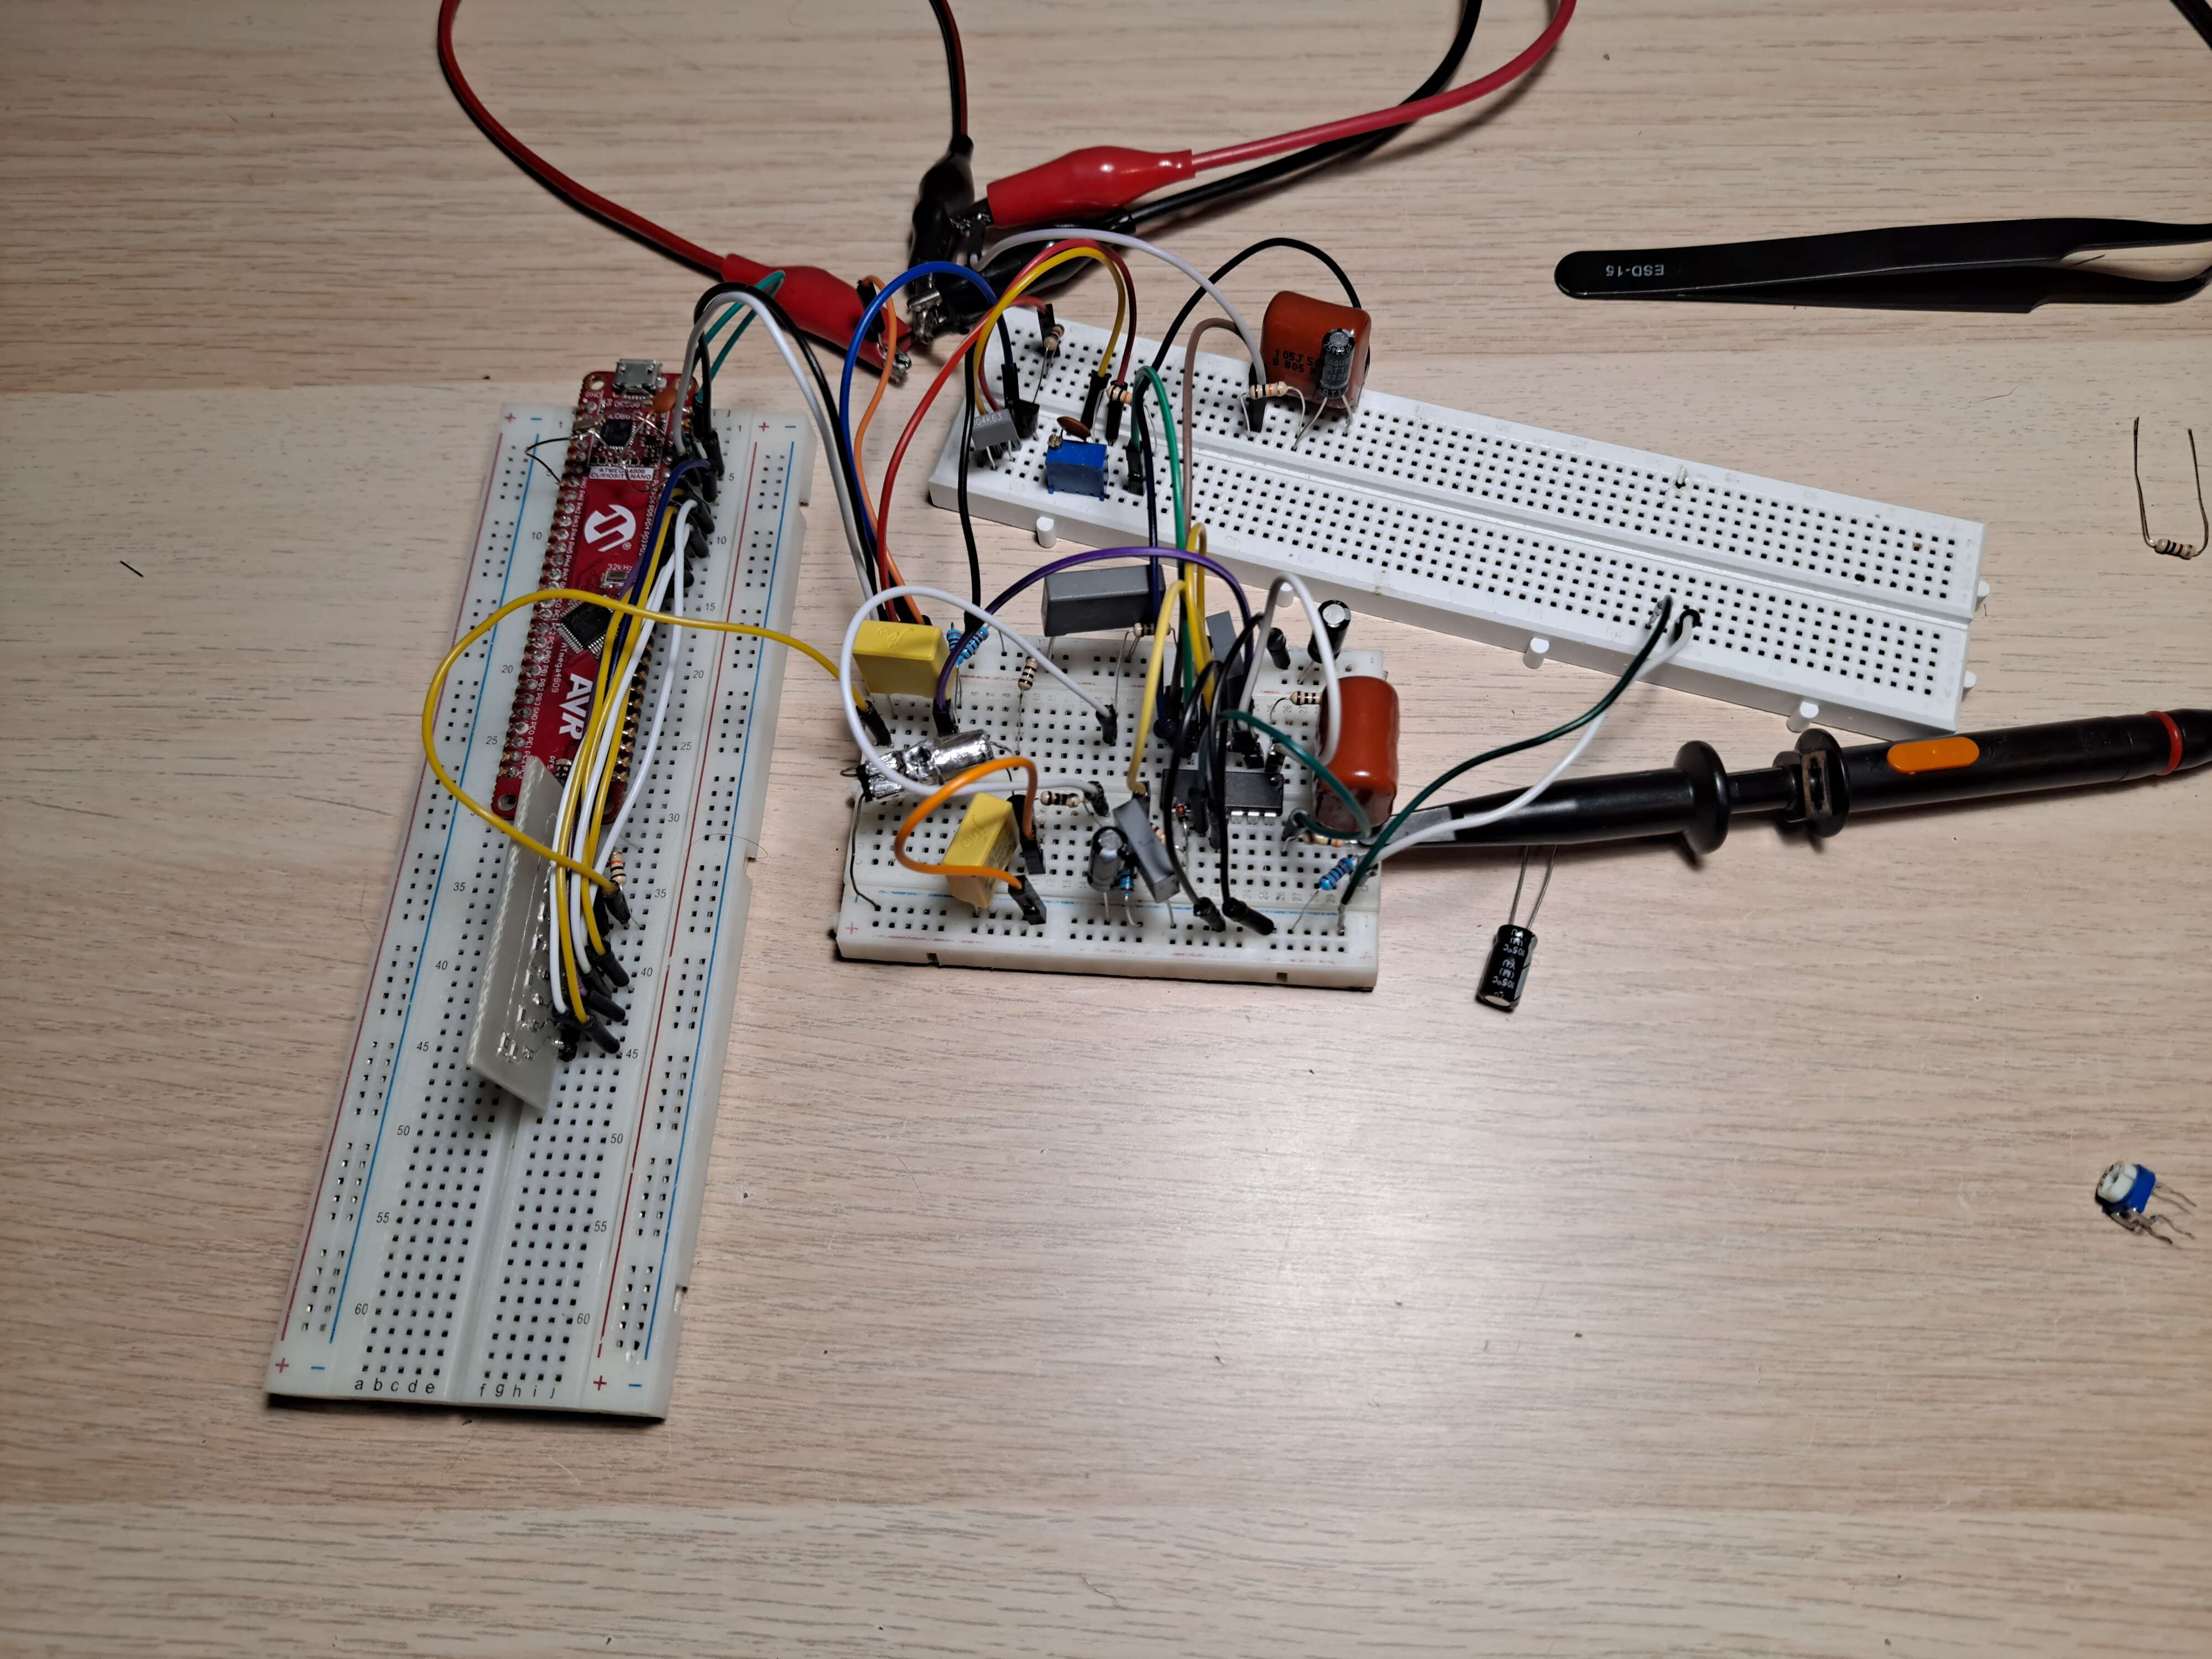
\includegraphics[width=0.8\textwidth]{img/experimental_setup.jpg}
	\caption{złożony układ eksperymentalny}
	
\end{figure}

Przedstawiony układ został przetestowany z następującymi różnicami względem schematu:

\begin{itemize}
	\item Mikrokontroler: ATMega4809
	\item Rezystory drabiny R-2R: \qty{10}{\kohm}, \qty{20}{\kohm}
\end{itemize}

Układ ATMega4809 zachowuje pełną kompatybilność kodu źródłowego z AVR32DA28,
gdyż oba mikrokontrolery bazują na tej samej wersji architektury AVR.

Generator w czasie pracy pobierał ok \qty{7}{\mA} Amplituda była poprawnie
kontrolowana oraz zachowywała stabilność przy zmiennym obciążeniu w zakresie \qty{1}{\kohm}-\qty{10}{\kohm}.
Układ stabilizował się po ok 1-2 sekundach od zmiany obciążenia.

Użyty oscyloskop nie pozwolił na użyteczny pomiar poziomu zniekształceń. 

\section{Schemat i płytka drukowana}

\newpage
\printbibliography[title=Źródła] %Prints bibliography

\newpage

\begin{figure}
	\centering
	
\includegraphics[width=0.75\textwidth]{img/kot_enter.jpg}
	\caption{Kot autora wspomagający proces twórczy}
\end{figure}

\end{document}